Results from model training and testing fell into three categories: loss, and perplexity, and subjective assessment of text output quality.

\subsection{Loss and Perplexity}
Best validation model loss, average test dataset loss and test dataset perplexity were collected for all tested models (see Figures \ref{best_loss}, \ref{avg_loss}, and \ref{perplexity}).
Loss and perplexity values were noticeably higher for the flash attention architecture on all models tested.

\begin{figure}[H]
    \centering
    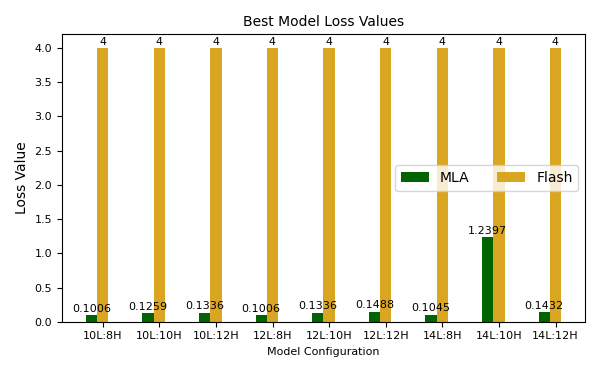
\includegraphics[width=\linewidth]{sections/images/best_loss.png}
    \caption{Best model loss for all tested models. L represents number of transformer layers. H represents number of attention heads.}
    \label{best_loss}
\end{figure}

\begin{figure}[H]
    \centering
    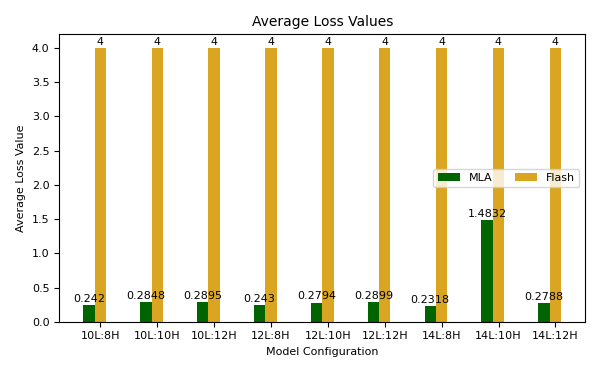
\includegraphics[width=\linewidth]{sections/images/avg_loss.png}
    \caption{Average model loss for all tested models. L represents number of transformer layers. H represents number of attention heads.}
    \label{avg_loss}
\end{figure}

\begin{figure}[H]
    \centering
    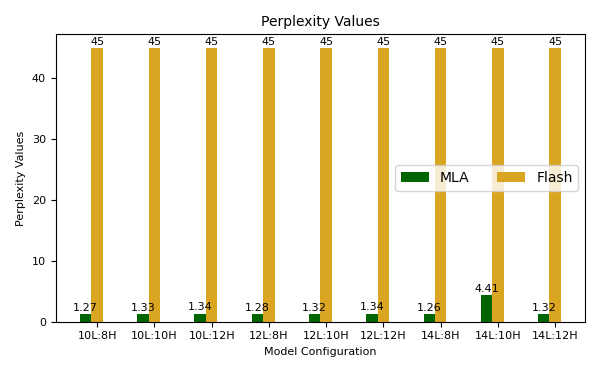
\includegraphics[width=\linewidth]{sections/images/perplexity.png}
    \caption{Perplexity loss for all tested models. L represents number of transformer layers. H represents number of attention heads.}
    \label{perplexity}
\end{figure}

\subsection{Subjective Assessment of Text Output Quality}
Text output from training and validation of each model configuration was reviewed by multiple team members. 
Several models were also provided custom prompts and output was assesed.
Taking into consideration factors such as sentence structure, text coherence, and word variability, the flash attention performed superiorly to MLA for all models tested\n.

General sentence flow and content for the flash attention model was readable and fairly coherent but generally lacked specificty and detail.  
Overall MLA models produced far less coherent text than the flash attention and contained may reptitions of a single word, which varied from model to model.
For MLA, models with higher loss and perplexity performed superiorly, suggesting a tendency for the models to overfit at the tested parameters.